\section{Terminology}
For the purpose of speaking the same language, this section introduces terminology required to understand the rest of this proposal.

\subsection{Technical Terms}
Understanding the construction of a new website requires familiarity with website terminology. Please remember that this reading is geared toward those with non-technical backgrounds, and does not require intimate knowledge of web technologies to understand.

The Internet is analogous to a highway: a series of roads that connect distinct locations, like your computer or mobile device, to other distinct locations, like websites and remote servers. Traveling on the highway is typically done using a web browser. Similar to a personal chauffer, a web browser prompts you for an address. Where do you want to go? That address is called the \textbf{Uniform Resource Locator (URL)}. These addresses are composed of several parts, but what matters for our purposes is the \textbf{domain name}. For instance, take this URL\@:

\begin{center}
    https://www.google.com/search?q=nyu+shanghai
\end{center}

The domain name is \textit{google.com}. Other examples of domain names are punahou.edu, minecraft.net, or onmagnoliasquare.com. Another term that often comes up is with the term domain name is \textbf{Top Level Domain (TLD)}, which just means the two to three letter segment after the dot. For example, edu, net, and com are all TLDs. For our domain,

\begin{center}
    https://www.onmagnoliasquare.com
\end{center}

The domain name is \textit{onmagnoliasquare.com}. The TLD is \textit{com}.

A \textbf{domain name registrar} provides domain name registration and leasing services. There are many domain name registrars, like GoDaddy, Namecheap, or Amazon Route 53. Domain names are leased on a yearly basis. Registrars often give the option to pay for two, five, or even 10 years in advance. Our current domain name registrar for OMS is GoDaddy.

Sometimes, domain name registrars offer \textbf{website hosting} services. For example, if a website was a building, some domain name registrars do not only let you register an address for your website, but they also lease a plot of land you can build your building on; they lease a physical space people can actually see and visit.

Now, imagine that the web browser is your personal chauffer once again. They take your provided URL address, https://onmagnoliasquare.com, and drive you to the OMS website. Before unlocking the doors and letting you off at the location, they check in with the security at the gates. Your chauffer wants to validate that the address you provided and your current location is indeed the place that you want to be. In other words, you gave your chauffer the address for the OMS website and now that you have arrived, they want to ensure that yes, this location is actually the OMS website, or no, this is not the OMS website, and the address you provided is wrongly associated with the current location. This validation is done with a \textbf{certificate}\footnote{In technical terms, this is called an SSL X.509 Domain Validated Certificate.}, a cryptographic electronic verification validating true ownership of a domain issued by a type of organization called a \textbf{Certificate Authority (CA)}. Your chauffer rolls down the window so location security can hand over their certificate for your chauffer to inspect. Upon inspection, your chauffer will either let you off or freak out. In the case that they freak out, it is most likely for this reason: the certificate from location security is a fraud! It is self-signed, meaning it was not issued by a valid CA\@. They turn to you and say: `Hey, there's an issue: your personal security may be at risk if I let you off at this location. After inspecting this location's certificate, it appears to be self-signed. Do you still want me to drop you off here?'

\begin{figure}[h]
    \centering
    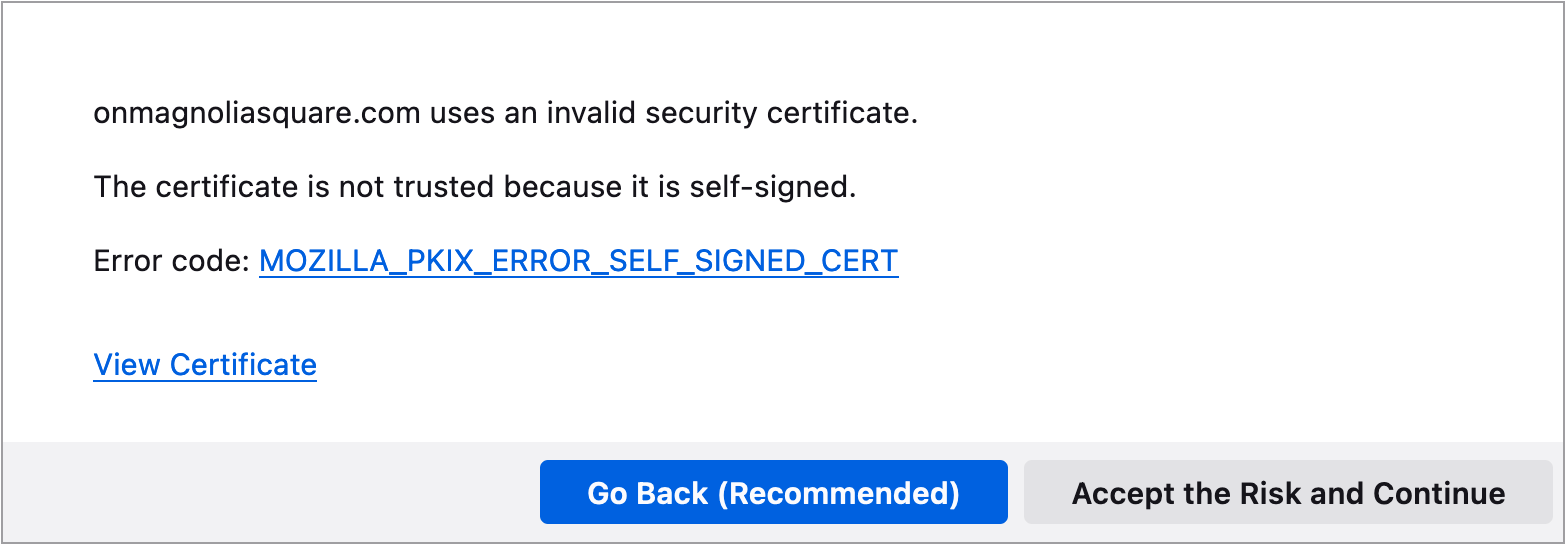
\includegraphics[scale=0.4]{pictures/chaufferexample1.png}
    \caption{A self-signed certificate warning in the Firefox web browser.}
    \label{fig:chauffer1}
\end{figure}

It is up to your discretion to exit the vehicle. Such a warning would scare off many people and tell their chauffer to bring them back home.

All the terms I have described thus far refer to the \textbf{backend}. It is infrastructure that our typical website reader is unaware of, nor needs to know anything about. Maintaining an online presence using a website is like hosting a theatrical play. You want an audience to come and watch. They do not care about the stagehands or the prop designers or even the words on the script or anything else happening off-stage. They care about the performance and the plot. They care about the \textbf{frontend}.

The frontend is typically associated with the term \textbf{User Interface and User Experience (UI/UX)}. It simply describes the qualities of the way a user of something interfaces with it, and the experience that accompanies using that interface.

For example, a wooden pencil has a simple user interface: a slightly long, cylindrical instrument beginning at a short rubbery stub, and terminating at a fine, cone-shaped tip. A pencil also has a non-problematic user experience: users can hold it in any which way they please without impairment to handwriting or drawing technique. These two characteristics of its UI/UX grant the user the ability to apply the graphite tip to a flat and markable medium in a sufficient and comfortable manner, such that any hand movements required to produce a writing or drawing can be done effectively, efficiently, and easily.

The content of many journals or newspaper websites, for example, the articles you read on JSTOR or The New York Times is created, updated, and deleted using a \textbf{content management system (CMS)}. A CMS interfaces between the frontend and the backend. It takes information from the backend, like articles or images, and sends them to be displayed at the frontend. A user who wants to update content on a website uses a CMS\@. A CMS is a tool developed for publishers, editors, and content creators, and so the UI/UX of a CMS is accessible for those genres of work.

A CMS can be imagined as the pencil in the UI/UX example. It interfaces between your brain and its ideas, and with the physical medium on which the idea will be presented. A CMS with a good UI/UX should feel fluent and fast, similar to how a pencil with a good UI/UX should feel comfortable and familiar.

\subsection{Qualitative Terms}
Each proposed backend and frontend service is chosen for its demonstration of good qualities in three categories of traits:

\begin{enumerate}
    \item Accessible
    \item Robust
    \item Future-proof
\end{enumerate}

Because of these traits, these services or tools can be used in the hands of a novice or experienced OMS member, with varying levels of technical ability, to achieve a satisfying outcome regardless of their goal.

\subsubsection*{Accessible}
Accessible backend services boast a user friendly UI/UX\@. The OMS members operating the website in the future must have a successful and satisfying experience. Malfunction should not result from bad design. Accessibility also means that technical literature on the service is easily accessible from online documentation, online forms, or tech support.

\subsubsection*{Robust}
 A robust service is one that must be able to be kicked and tossed to the ground without compromise to its dependability. It is also mistake agnostic – an ignorant mistake or a well conceived blunder by an OMS member using the service will not hinder the service's reliability to display the website to our audience. In the case where an issue occurs, information to fix it is readily accessible.

 Robust services also beget high standards of security, in the form of accessible user access management systems, multi-factor authentication, or reliable customer support.

\subsubsection*{Future-proof}
Regardless of a service's accessibility and robustness, if it will not exist in the future, it is not employable in the present. Future members members must be able to access and use the service. I have chosen services created by strong and reputable companies in their respective technical circles, such that if a breaking change for their customers were to ever emerge down the line, a warning or notice will have been announced several months beforehand. This gives time for members to explore other service solutions.
